\documentclass[a4paper,titlepage,onecolumn,table]{article}

% Title Page
\title{Data Science Methods - Homework 1}
\author{Hans de Ferrante}
\usepackage[margin=1.25in]{geometry}
\usepackage[]{mathtools}
\usepackage{graphicx}
\graphicspath{ {Images/}}
\usepackage{float}
\usepackage{placeins}

\usepackage{kbordermatrix}
\usepackage{amsmath}
\usepackage{amssymb}
\usepackage[amsmath,amsthm,thmmarks]{ntheorem}

\usepackage{graphicx}
\newcommand{\indep}{\rotatebox[origin=c]{90}{$\models$}}

\usepackage[table]{xcolor}
\usepackage{tikz}
\usepackage[final]{pdfpages}
\usetikzlibrary{arrows}

\newcommand*\circled[1]{\tikz[baseline=(char.base)]{\node[shape=circle,draw,inner sep=2pt] (char) {#1};}}

\renewcommand{\kbldelim}{(}% Left delimiter
\renewcommand{\kbrdelim}{)}% Right delimiter

\newcommand\x{\times}
\newcommand\y{\cellcolor{green!30}}
\newcommand\yy{\cellcolor{blue!20}}
\newcommand\yyy{\cellcolor{purple!20}}

\begin{document}
	
	\section*{Homework 2 - Data Science Methods}
	Hans de Ferrante, 910957
	
	\section{Question 1: Lasso \& Ridge}
	\textit{a) Explain what Lasso and Ridge tend to do to the coefficients of two highly correlated variables in a linear model.}\\[0.2cm]
	\par First, let us start by stating the obvious: Lasso and Ridge are both shrinkage methods. This will mean that both methods will tend to decrease the average norm of the coefficient estimates as $\lambda$ increases. One important difference between the two is that Lasso will set some coefficients explicitly to zero if we increase the tuning parameter $\lambda$ ("Lasso kicks out"), whereas Ridge will simply keep shrinking both coefficients proportionally. This effectively means that Lasso will tend to select only one of the highly correlated variables for large $\lambda$, whereas Ridge will keep both coefficients. \\[0.2cm]
	
	\textit{b) Does Lasso select the (true non-zero) regressors with probability one as the sample grows large? Explain.} \\[0.2cm]
	\par
	I don't think we have discussed this at length in the lectures (although we did see that for the adaptive lasso this result holds since adaptive lasso satisfies the oracle properties and consistent variable selection is one of these properties). On the slides, however, it is briefly mentioned that indeed Lasso is able to select the true model with probability one as the sample grows large provided that the true model is sparse and has $p$ not too large compared to $n$. I did not recall having discussed this in the lecture so I decided to consult the literature on Lasso. I found it quite technical and difficult to understand but hope I understood it correctly.
	\par
	In this literature, authors make the distinction between (i) estimation consistency and (ii) model consistency of Lasso (e.g. Zhao2006). With regards to (i) it has been shown that under mild regularity conditions Lasso is indeed estimation consistent. Hence, we can expect the zero regressor coefficient estimates to converge in probability to 0 as $n \rightarrow \infty$. (ii) is more tricky and requires the Irrepresentable Condition, variations of which have been derived independently by different authors. These include Zhao2006, Zou2006 and Meinshausen2006. Zhao2006 is a highly cited paper that provides a simple example of a case where the condition does not hold, and consequently Lasso is unable to select the correct model \cite{Zhao:2006:MSC:1248547.1248637}. The example works with $n=1000$ and $p=3$ so I do think it presents a situation where $n$ grows large compared to $p$ as we assumed in the question.
	\par
	I find it therefore difficult to come up with a non-ambiguous answer to this question as the answer depends on how we define Lasso selecting the true non-zero regressors with probability one as the sample grows large. As $n \rightarrow \infty$ the zero regressors will converge to 0 so for sure we will know which regressors are truly non-zero and which are not in the limit. However, we would need to check the Irrepresentable Condition to verify whether Lasso would truly kick out non-zero regressors (arbitrarily close to 0 is not 0). Downside is that this is practically impossible as we would need the true covariance matrix for checking the condition. \\[0.2cm]	
	\textbf{Long story short}: If we only need estimation consistency, yes: zero coefficients converging to 0 is established result. If we want model consistency in the sense that we want Lasso to kick all zero regressors out, not generally; we would need to verify IC.
	
	\bibliography{bib}
	\bibliographystyle{apalike}
		
	\section{Question 2}
	\textit{Prove that the $l2$-norm $||\hat{\beta}_{RIDGE}||$ of the ridge estimates $\hat{\beta}_{RIDGE}$ from a ridge regression of $y$ on $X$ ($n \times p$ full rank matrix, with $p<n$) is always decreasing in $\lambda$.} \\[0.2cm]
	\par
	Recall from the LN that $\hat{\beta}_{RIDGE} = (X'X+\lambda I)^{-1}X'y$. Note that under the assumptions $p<n$ and $X$ $(n\times p)$ full rank, we can use the SVD for $X$, i.e. $X=UDV'$ with $U$ and $V$ unitary matrices, $D$ a diagonal matrix with diagonal entries $d_{ii}>0 \quad \forall \quad i, 0$ otherwise. This implies in particular $D'$ = $D$, $U'U = I_p$, and $V'=V^{-1}$. Hence, we can rewrite	
	\begin{align*}
	\hat{\beta}_{RIDGE} & = [(UDV')'UDV'+\lambda I]^{-1}(UDV')'y = (VD'U'UDV'+\lambda I)^{-1}VD'U'y \\ 
	& = (VD'U'UDV'+\lambda I)^{-1}VD'U'y = (VD^2V'+\lambda I)^{-1}VDU'y =\\
	& = (VD^2V'+\lambda VV')^{-1}VDU'y = (V(D^2+\lambda I)V')^{-1}VDU'y = \\
	& = (V')^{-1}(D^2+\lambda I)^{-1}V^{-1}VDU'y = V(D^2+\lambda I)^{-1}V^{-1}VDU'y = \\
	& = V(D^2+\lambda I)^{-1}DU'y.
	\end{align*}
	where we use in addition to the mentioned implications the following (trivial) results from linear algebra:
	\begin{align*}
	& (ABC)^{-1} = C^{-1}B^{-1}A^{-1}  \qquad \& \qquad (ABC)' = C'B'A'.
	\end{align*}
	
	Now we know that by definition for the $l_2$-norm of vectors, we can write $||\hat{\beta}_{RIDGE}||^2 = \hat{\beta}_{RIDGE}'\hat{\beta}_{RIDGE}$. If we plug in the expression above, we find therefore:
	\begin{align*}
	||\hat{\beta}_{RIDGE}||^2 &=  (V(D^2+\lambda I)^{-1}DU'y)'V(D^2+\lambda I)^{-1}DU'y \\
	& = (U'y)'D((D^2+\lambda I)^{-1})'V'V(D^2 + \lambda I)^{-1}DU'y \\
	& = (U'y)'D(D^2+\lambda I)^{-1}(D^2 + \lambda I)^{-1}D(U'y) \\
	& = x'Ax
	\end{align*}
	where the last equality shows that this is a quadratic form with $A = D^2(D^2+\lambda I)^{-2}$ and $x = U'y$. Now getting rid of the matrix notation, we see that 
	\begin{equation*}
	||\hat{\beta}_{RIDGE}||^2 = 
	\begin{bmatrix}
	x_1 & x_2 & \hdots & x_p 
	\end{bmatrix}
	\begin{bmatrix}
	\frac{d_{11}^2}{(d_{11}^2+\lambda)^2}       & 0  & \dots & 0 \\
	0       & \frac{d_{22}^2}{(d_{22}^2+\lambda)^2}  & \dots & 0 \\
	\vdots  & \vdots & \ddots & 0 \\
	0 & 0 & 0 & \frac{d_{pp}^2}{(d_{pp}^2+\lambda)^2}
	\end{bmatrix}
	\begin{bmatrix}
	x_1 \\ x_2 \\ \vdots \\ x_p 
	\end{bmatrix}
	= \frac{x_1^2d_{11}^2}{(d_{11}^2+\lambda)^2} + \hdots + \frac{x_p^2d_{pp}^2}{(d_{pp}^2+\lambda)^2}
	\end{equation*}
	It is trivial to see from this final equation that this final equation is decreasing in $\lambda$ as all numerators increase in $\lambda$ and denominators remain the same. This implies that  $||\hat{\beta}_{RIDGE}|| = \sqrt{||\hat{\beta}_{RIDGE}||^2}$ is too decreasing in $\lambda$ as the square root transformation is a monotonic one.
	

	\hspace{-.1\linewidth}
	
	
	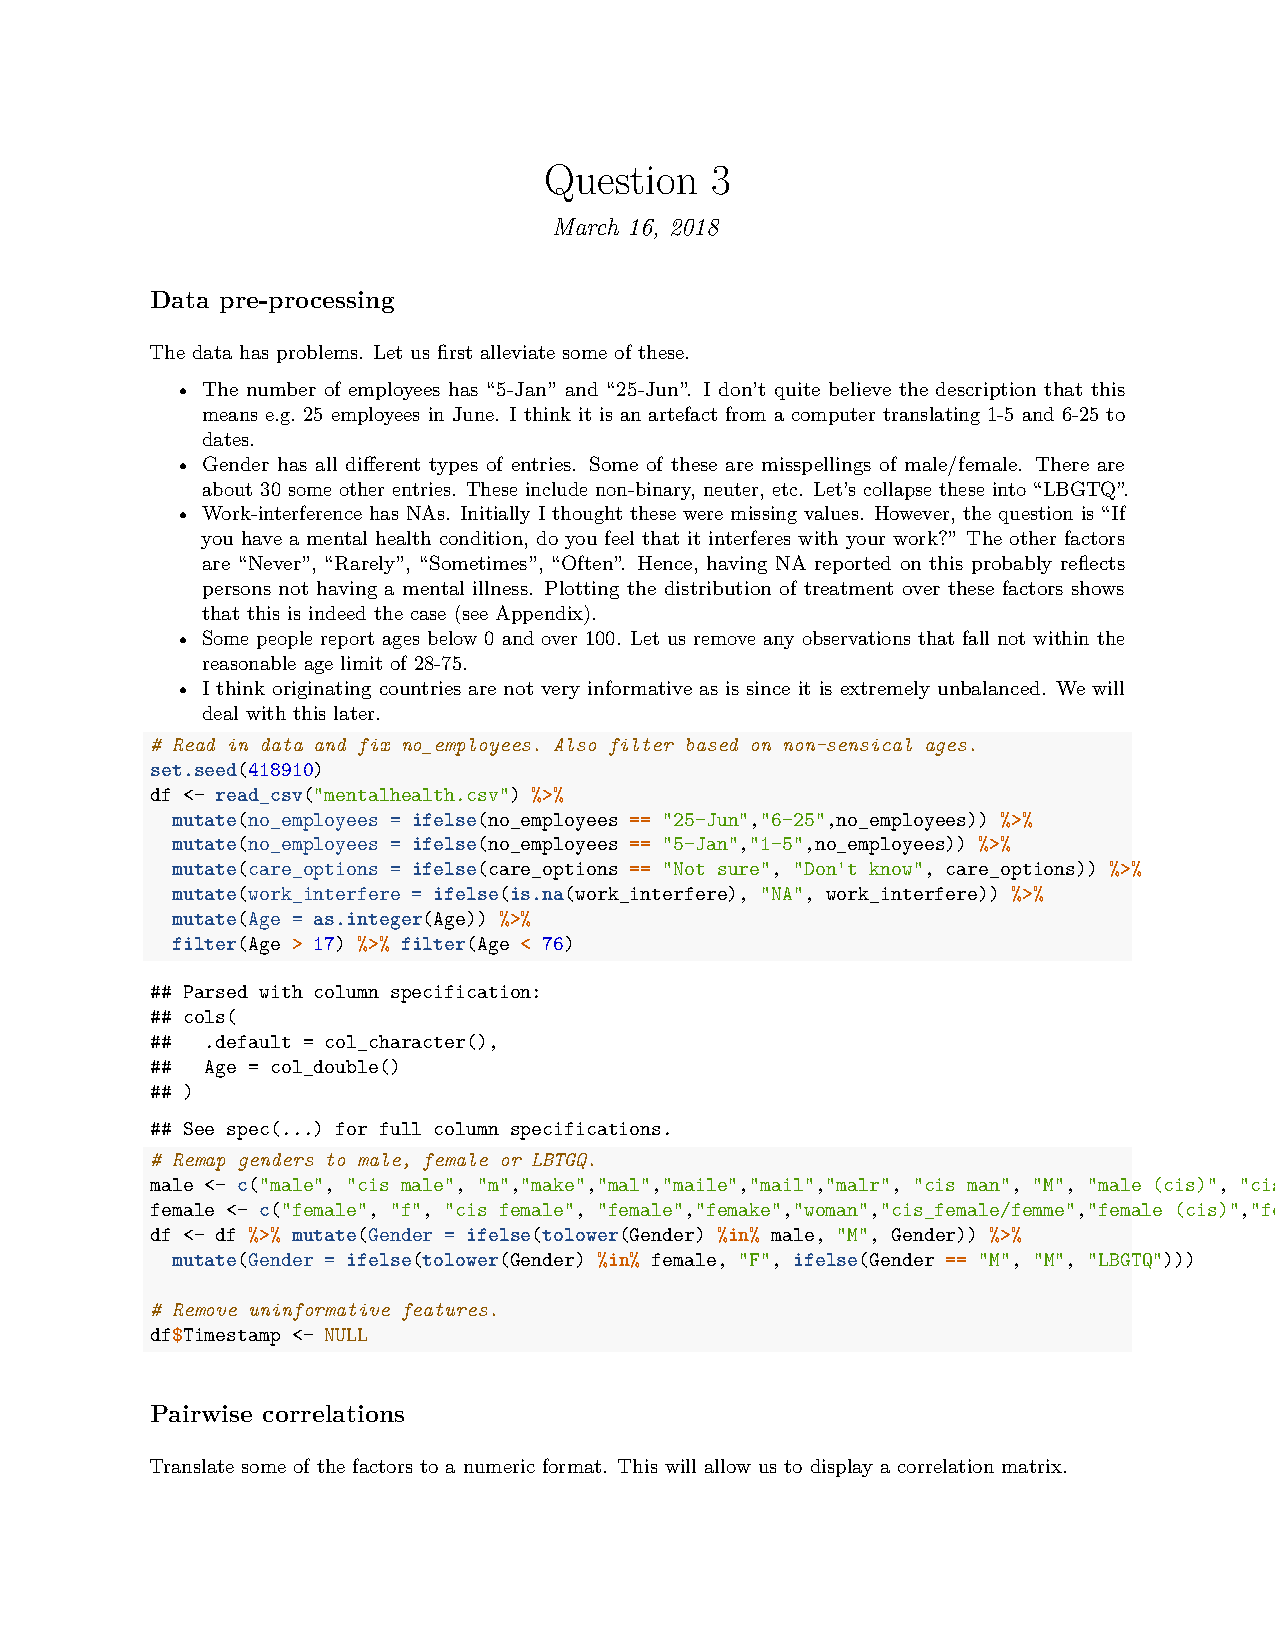
\includepdf[pages=-,pagecommand={},width=1.3\linewidth]{../Assignment2.pdf}
	
\end{document}